\documentclass[a4paper, 11pt]{article}
\usepackage[polish]{babel}
\usepackage[T1]{fontenc}
\usepackage{hyperref}
\usepackage{array}
\usepackage{amssymb}
\usepackage{amsmath}
\usepackage{changepage}
\usepackage{multicol}
\usepackage[margin=1in]{geometry}
\hypersetup{
    colorlinks,
    citecolor=black,
    filecolor=black,
    linkcolor=black,
    urlcolor=black
}
\usepackage{graphicx}

\usepackage{tikz}
\usetikzlibrary{fit,arrows,matrix,positioning, calc, shapes.gates.logic.IEC, shapes.gates.logic.US}
\usetikzlibrary {arrows.meta}
\tikzstyle{branch}=[fill,shape=circle,minimum size=3pt,inner sep=0pt]


\title{%
        \vspace{-1cm}
       \large Sprawozdanie Laboratorium Fizyka dla informatyków \\
       \huge Wyznaczanie współczynnika rozszerzalności liniowej ciał stałych.}

\author{Stanisław Fiedler 160250}
\date{LAB 2, 12 listopada 2024}

\begin{document}
\begin{table}
	\begin{adjustwidth}{-0.25\textwidth}{-0.25\textwidth}
		\begin{center}
			\begin{tabular}{|l|l|l|l|l|}
				\hline
				Nr Ćwiczenia 103                                             & Data wykonania 12.11.2024                 & Wydział WIiT & Semestr 3 & Grupa LAB L1 \\
				\hline
				\multicolumn{2}{|l|}{ Prowadzący: mgr inż. Taras Zhezhera  } & \multicolumn{2}{|l|}{ Stanisław Fiedler } & Ocena:                                  \\
				\hline
			\end{tabular}
		\end{center}
	\end{adjustwidth}
\end{table}

\maketitle
\tableofcontents

\section{Wstęp teoretyczny}\label{sec:wstep} % (fold)
Zmianie temperatury ciała towarzyszy na ogół zmiana jego wymiarów linowych,
a więc także zmiana jego objętości.
Przyrost temperatury $dT$ ciała, którego długość całkowita wynosi l,
powoduje przyrost długości $dl$ określony wzorem:
\begin{equation}\label{eq:alpha1}
	dl = \alpha l\,dT
\end{equation}
Współczynnik $\alpha$ nazywamy współczynnikiem rozszerzalności liniowej.
W zakresie niewielkich zmian temperatury możemy przyjąć, że współczynnik $\alpha$ jest stały,
a długość wzrasta wprost proporcjonalnie do temperatury.
W tym przypadku odpowiednikiem wzoru \eqref{eq:alpha1} jest wzór:
\begin{equation}\label{eq:alpha2}
	l - l_0 = \alpha_{sr}l_o \Delta T
\end{equation}
\begin{equation}\label{eq:alpha3}
	\alpha_{sr} = \frac{l - l_0}{l_0 \Delta T}
\end{equation}

Przyczyna rozszerzalności cieplnej leży w strukturze mikroskopowej ciał.
Ciała zbudowane są z atomów tworzących sieć krystaliczną.
Dostarczona energia cieplna powoduje drgania atomów wokół położeń równowagi.
Amplituda tych drgań rośnie wraz z temperaturą.
Wraz ze wzrostem amplitudy drgań roście średnia odległość między atomami co obserwujemy jako rozszerzalność cieplna.

% section wstep (end)

\section{Wyniki pomiarów}\label{sec:wyniki_pomiarow} % (fold)

\begin{center}
	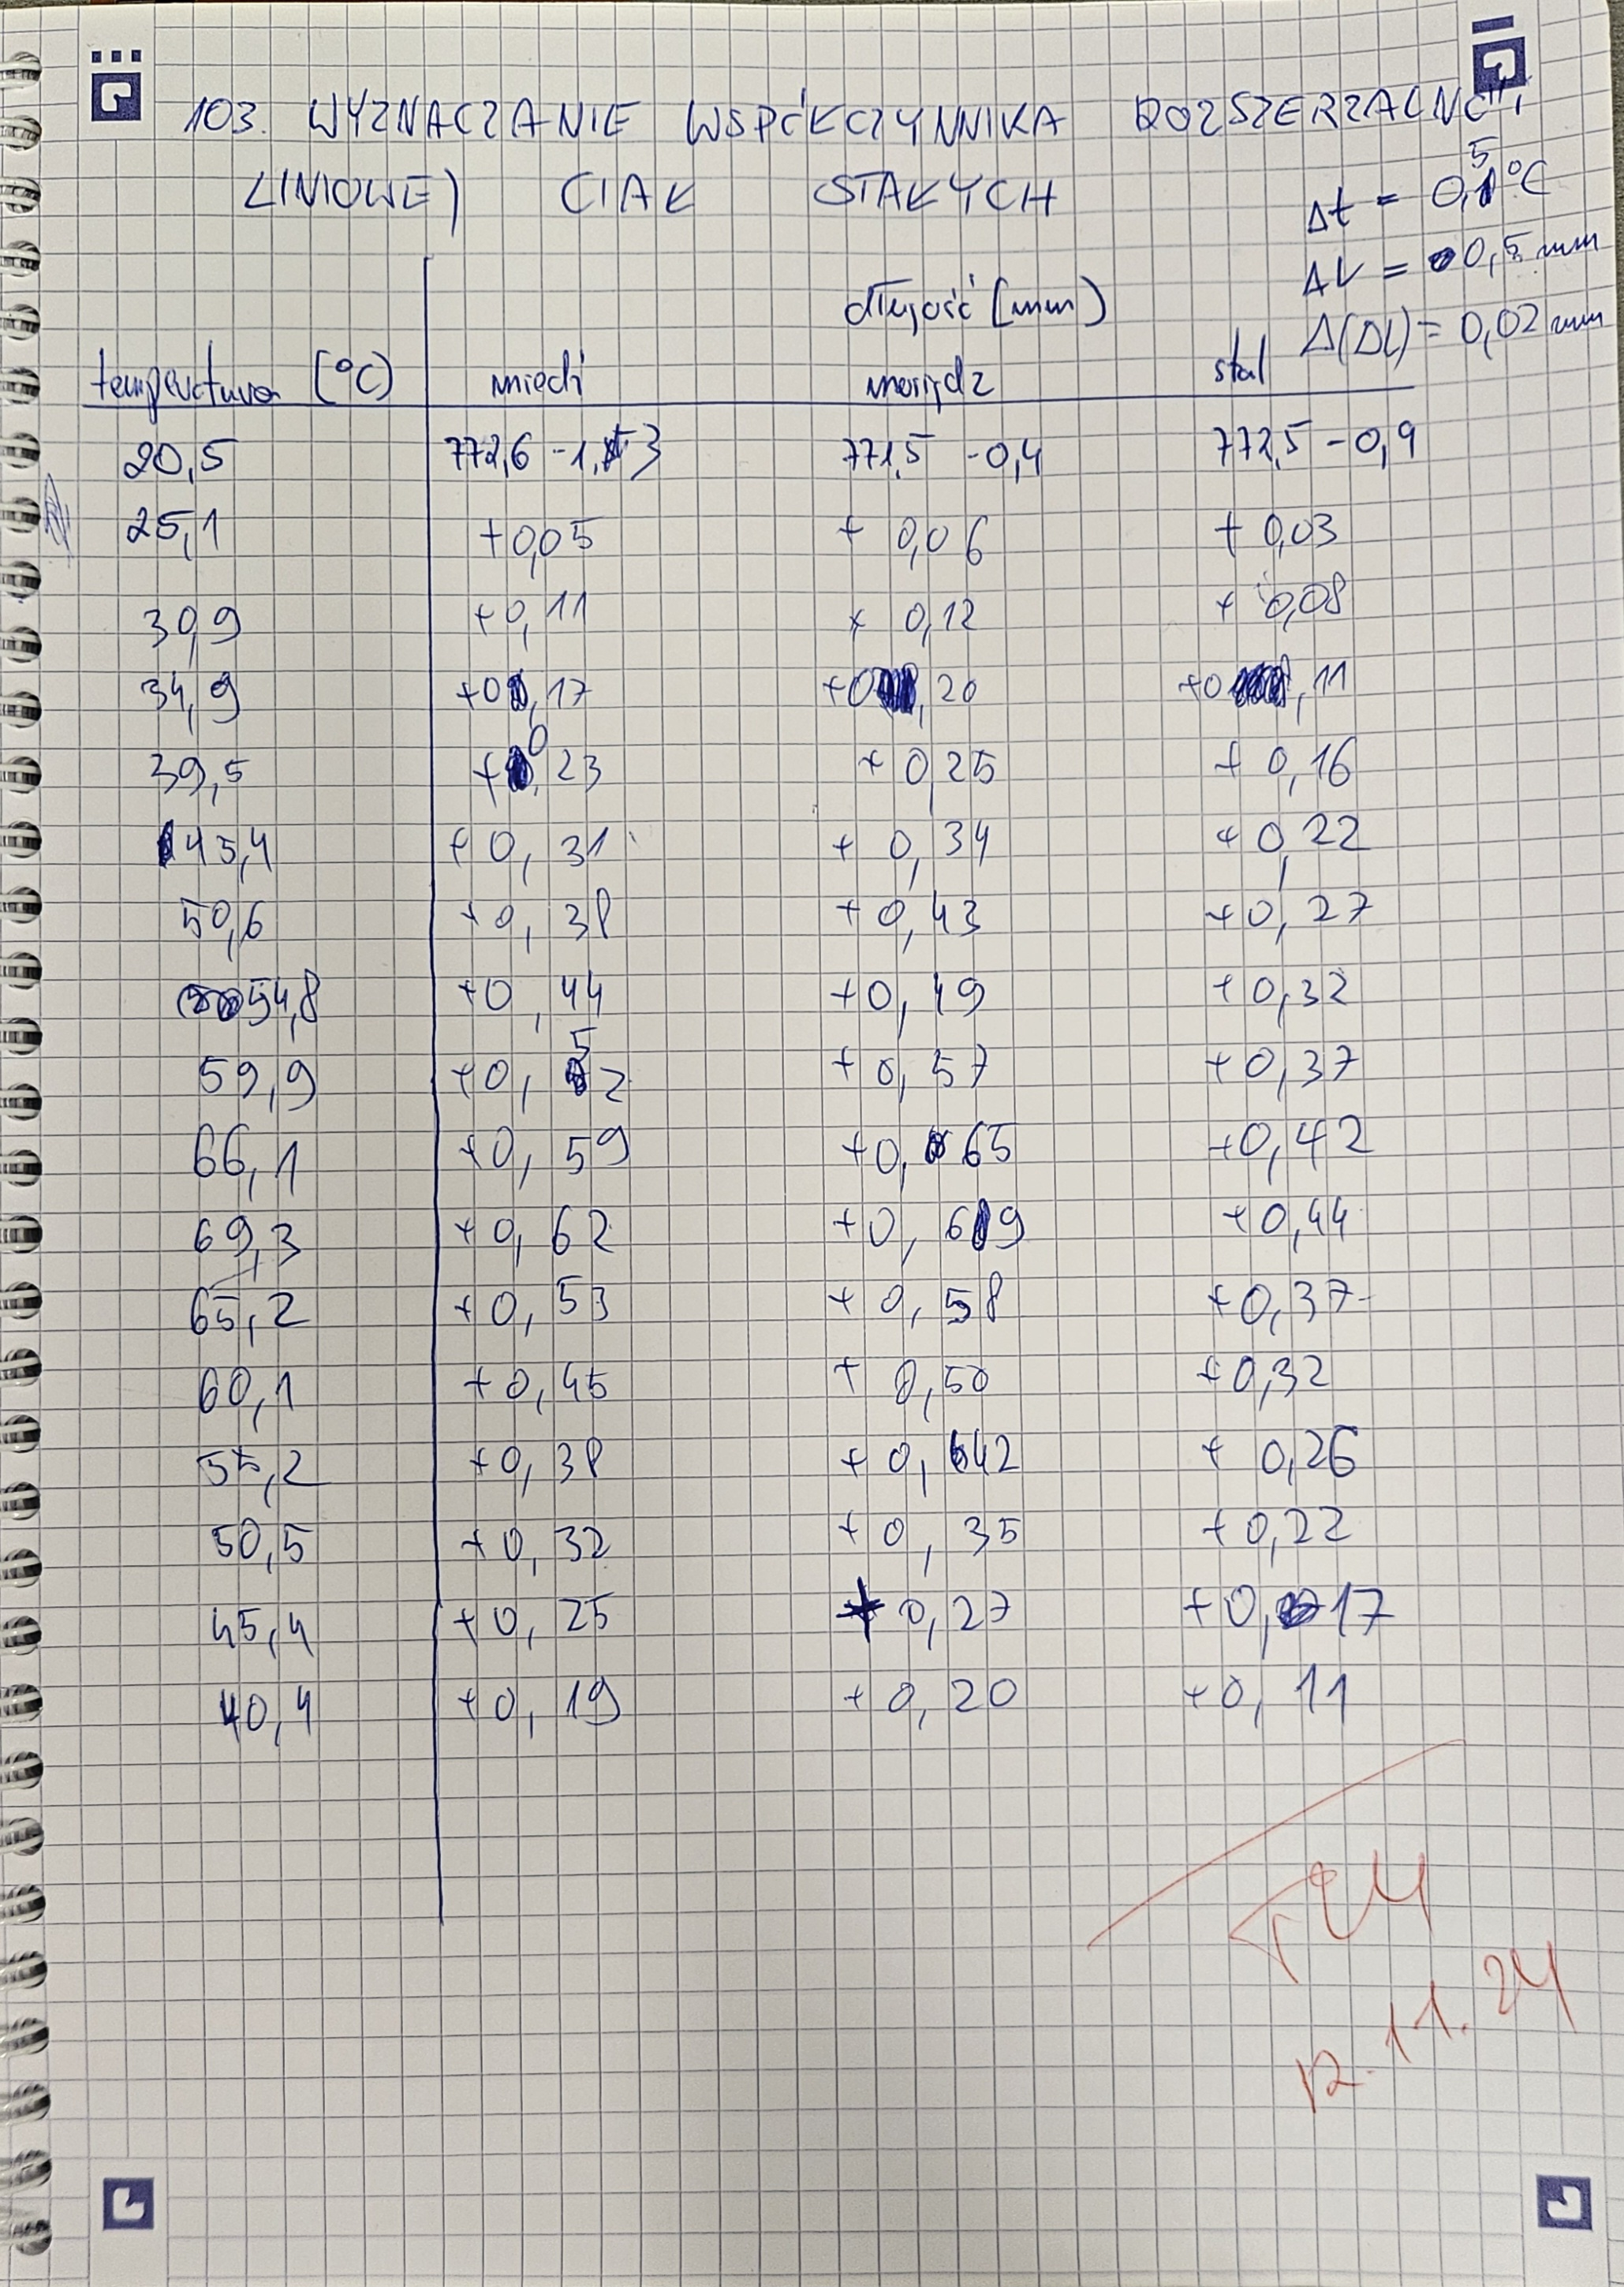
\includegraphics[scale=0.22]{images/pomiary.jpg}
\end{center}
% subsection Zdjecie wynikow pomiarow (end)

\pagebreak
\section{Opracowanie wyników}\label{sec:opracowanie_wynikow} % (fold)

\subsection{Wykres}\label{sub:wykres} % (fold)
\begin{center}
	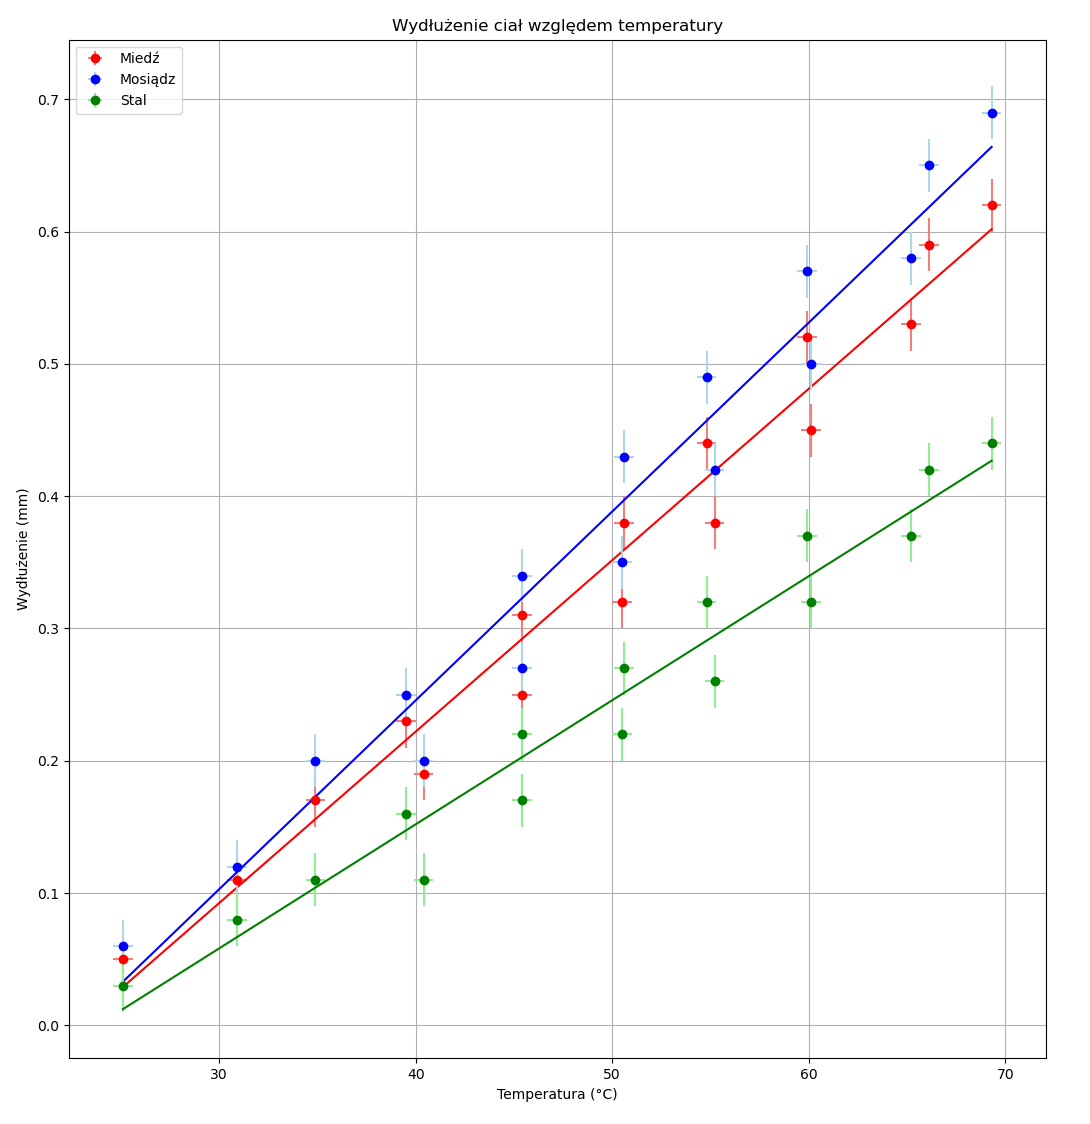
\includegraphics[scale=0.3]{images/wykres2.png}

	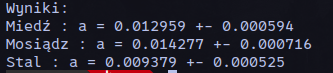
\includegraphics[scale=0.7]{images/wyniki.png}
\end{center}

Regresja liniowa oraz jej błąd zostały wyznaczone w python z użyciem biblioteki scipy.

% subsection Wykres (end)

\subsection{Obliczenia}\label{sub:obliczenia} % (fold)
W celu wyznaczenia współczynnika rozszerzalności z danych pomiarowych zapiszemy równanie \eqref{eq:alpha2} w postaci:
\begin{equation}
	\Delta l = \alpha_{sr} l_0 T - \alpha_{sr} l_0 T_0
\end{equation}
Równanie to oznacza, że wydłużenie jest linową funkcją temperatury i że współczynnik nachylenia prostej
$a = \alpha_{sr}l_0$ . Więc współczynnik rozszerzalności wyznaczymy ze wzoru:
\begin{equation}
	\alpha = \frac{a}{l_0}
\end{equation}

Błąd zostanie obliczony z użyciem  metody różniczki logarytmicznej na podstawie
niepewności współczynnika nachylenia regresji liniowej oraz niepewności pomiaru długości.

\[
	\alpha = a^1 \cdot l_0^{-1}
\]
\[
	\Delta \alpha = \left( \frac{\Delta a}{a} + \frac{\Delta l_0}{l_0} \right) \alpha
\]

\subsubsection{Długości początkowe i niepewności}

\begin{multicols}{2}

	Początkowa długość prętów:
	\begin{itemize}
		\item Miedź 772,6 - 1,3 = 771,3mm
		\item Mosiądz 771,5 - 0,4 = 771,1 mm
		\item Stal 772,5 - 0,9 = 771,6 mm
	\end{itemize}

	\columnbreak

	Niepewności pomiarowe:
	\begin{itemize}
		\item $ \Delta T = 0,5^{\circ}C$
		\item $ \Delta l = 0,5mm $
		\item $ \Delta(\Delta l) = 0,02mm  $
	\end{itemize}

\end{multicols}
% subsection Obliczenia (end)

\subsubsection{Miedź}\label{sub:miedz} % (fold)
Równanie prostej:
\[
	a = 0,0129592 \pm 0,0005936
\]
\begin{multicols}{2}
	\[
		\alpha_{miedz} = \frac{a}{l_0}
	\]
	\[
		\alpha_{miedz} = \frac{0,0129592}{771,3} \quad \frac{1}{K}
	\]
	\[
		\alpha_{miedz} = 1.6801 \cdot 10^{-5} \quad \frac{1}{K}
	\]
	\columnbreak
	\[
		\Delta \alpha = \left( \frac{\Delta a}{a} + \frac{\Delta l_0}{l_0} \right) \alpha
	\]
	\[
		\Delta \alpha = \left( \frac{0,0005936}{0,0129592} + \frac{0,05}{771,3} \right) 1.6801763 \cdot 10^{-5}\quad \frac{1}{K}
	\]
	\[
		\Delta \alpha = 0,077 \cdot 10^{-5}\quad \frac{1}{K}
	\]
\end{multicols}
% subsection Miedz (end)

\subsubsection{Mosiądz}\label{sub:mosiadz} % (fold)
Równanie prostej:
\[
	a = 0,014277 \pm 0.000716
\]
\begin{multicols}{2}
	\[
		\alpha_{mosiadz} = \frac{a}{l_0}
	\]
	\[
		\alpha_{mosiadz} = \frac{0,014277}{771,1} \quad \frac{1}{K}
	\]
	\[
		\alpha_{mosiadz} = 1.85151 \cdot 10^{-5} \quad \frac{1}{K}
	\]
	\columnbreak
	\[
		\Delta \alpha = \left( \frac{\Delta a}{a} + \frac{\Delta l_0}{l_0} \right) \alpha
	\]
	\[
		\Delta \alpha = \left( \frac{0.000716}{0,014277} + \frac{0,05}{771,1} \right) 1.85151 \cdot 10^{-5}\quad \frac{1}{K}
	\]
	\[
		\Delta \alpha = 0.093 \cdot 10^{-5}\quad \frac{1}{K}
	\]
\end{multicols}
% subsection Mosiadz (end)

\subsubsection{Stal}\label{sub:stal} % (fold)
Równanie prostej:
\[
	a = 0,009379 \pm  0.000525
\]
\begin{multicols}{2}
	\[
		\alpha_{stal} = \frac{a}{l_0}
	\]
	\[
		\alpha_{stal} = \frac{0,009379}{771,6} \quad \frac{1}{K}
	\]
	\[
		\alpha_{stal} = 1.2155 \cdot 10^{-5} \quad \frac{1}{K}
	\]
	\columnbreak
	\[
		\Delta \alpha = \left( \frac{\Delta a}{a} + \frac{\Delta l_0}{l_0} \right) \alpha
	\]
	\[
		\Delta \alpha = \left( \frac{0.000525}{0,009379} + \frac{0,05}{771,6} \right) 1.2155 \cdot 10^{-5}\quad \frac{1}{K}
	\]
	\[
		\Delta \alpha = 0.0681 \cdot 10^{-5}\quad \frac{1}{K}
	\]
\end{multicols}
% subsection Stal (end)

\pagebreak
\subsection{Wyniki}\label{sub:wyniki} % (fold)

\begin{center}
	\Large
	Miedź
	\[
		\alpha = (1,68 \pm 0,07)  \cdot 10^{-5} \quad \frac{1}{K}
	\]
	Mosiądz
	\[
		\alpha = (1,85 \pm 0,09)  \cdot 10^{-5} \quad \frac{1}{K}
	\]
	Stal
	\[
		\alpha = (1,22 \pm 0,07) \cdot 10^{-5} \quad \frac{1}{K}
	\]
\end{center}

% subsection Wyniki (end)

\subsection{Wnioski}\label{sub:wnioski} % (fold)
Wartości tablicowe współczynników rozszerzalności linowej, podane za \href{https://openstax.org/books/fizyka-dla-szk%C3%B3%C5%82-wy%C5%BCszych-tom-2/pages/1-3-rozszerzalnosc-cieplna}{openstax.org}
, wynoszą dla:
\begin{description}
	\item[Miedź] $ 1,7 \cdot 10^{-5} \frac{1}{K}$
	\item[Mosiądz] $ 1,9 \cdot 10^{-5} \frac{1}{K}$
	\item[Stal] $ 1,2 \cdot 10^{-5} \frac{1}{K}$
\end{description}
Jak widać wyznaczone wartości zgadzają się z wartościami tablicowymi, a powstałe różnice mogą wynikać z różnic między proporcjami składników w stopach stali i mosiądzu.
% subsection Wnioski (end)

\end{document}

